\documentclass[12pt]{amsart}

\usepackage{a4wide, amsxtra}

\usepackage[pdftex]{graphicx}

 \title{PMTH212 Assignment 2}

 \author{Mark Villar}

\begin{document} 

\maketitle 

\begin{enumerate}
	
	\item The surface is a hyperboloid of 1 sheet with centre $(-1,1,2)$.
		\begin{align*}
			z^2-4z&=4x^2+8x+y^2-2y \\
			(z-2)^2-4&=4(x^2+2x)+(y-1)^2-1 \\
			(z-2)^2&=4\big[(x+1)^2-1\big]+(y-1)^2+3 \\
			(z-2)^2&=4(x+1)^2+(y-1)^2-1 \\
			1&=4(x+1)^2+(y-1)^2-(z-2)^2
		\end{align*}
		\begin{figure}[h]
					\centering
					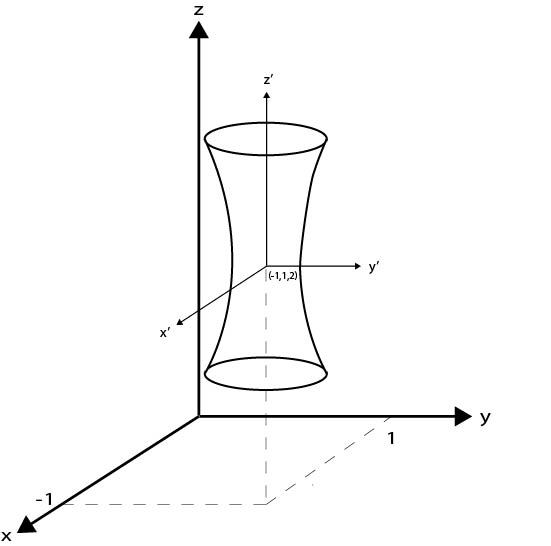
\includegraphics[width=5in]{Hyperboloid.jpg}
				\end{figure}
	\item The orthogonal projection onto the $xy$-plane of the curve of intersection is given by
		\begin{align*}
			z=4-x^2-y^2=y^2 \ \Rightarrow \ x^2+2y^2=4
		\end{align*}
		Since this equation does not contain $z$ the projection is a cylindrical surface. \\
				
	\item 
	
		\begin{enumerate}
		
			\item The graph is a circle with radius 3 and centre $(0,0)$.
				\begin{align*}
					&x=3\sin2t, \ \ \ y=3\cos2t \\
					&x^2+y^2=9\sin^22t+9\cos^22t=9 \\
					&(x-0)^2+(y-0)^2=3^2
				\end{align*}
			
			\item The graph is a parabola with vertex $(y,z)=(0,-1)$ which lies on the plane $x=-2$.
				\begin{align*}
					&x=-2, \ \ y=t, \ \ z=t^2-1 \ \Rightarrow \ z=y^2-1
				\end{align*}
		
		\end{enumerate}
				
	\item $\mathbf{r}$ is a smooth curve of the parameter $t$ since $\mathbf{r}'(t)$ exists and is continuous 			and $\mathbf{r}'(t)\ne0$ for all $t$. We examine the components of $\mathbf{r}'(t)$ to confirm this.
		\begin{align*}
			&x(t)=\cos t^2, \ \ \ y(t)=\sin t^2, \ \ \ z(t)=e^{-t} \\
			&x'(t)=-2t\sin t^2, \ \ y'(t)=2t\cos t^2, \ \ z'(t)=-e^{-t} \\
			&\mathbf{r}'(t)=(-2t\sin t^2)\mathbf{i}+(2t\cos t^2)\mathbf{j}+(-e^{-t})\mathbf{k}
		\end{align*}
		Since $-2t\sin t^2$, \ $2t\cos t^2$, \ $-e^{-t}$ \ are all continuous functions of $t$, then $\mathbf{r}'(t)$ \ 		is also continuous. Moreover,
		\begin{align*}
			x'(t)^2+y'(t)^2+z'(t)^2=4t^2+e^{-2t} > 0 \ \text{for all} \ t
		\end{align*}
		Hence, there is no value of $t$ for which all three components are zero.
	\item
		\begin{align*}
			\frac{d }{dt}\big[\mathbf{u}\cdot(\mathbf{v}\times\mathbf{w})\big]&=\frac{d\mathbf{u}}{dt}\cdot
			(\mathbf{v}\times\mathbf{w})+\mathbf{u}\cdot\frac{d(\mathbf{v}\times\mathbf{w})}{dt} \\
			&=\frac{d\mathbf{u}}{dt}\cdot\big[\mathbf{v}\times\mathbf{w}\big]+\mathbf{u}\cdot\Big[\mathbf{v}
			\times\frac{d\mathbf{w}}{dt}+\frac{d\mathbf{v}}{dt}\times\mathbf{w}\Big] \\
			&=\frac{d\mathbf{u}}{dt}\cdot\big[\mathbf{v}\times\mathbf{w}\big]+\mathbf{u}\cdot\Big[
			\frac{d\mathbf{v}}{dt}\times\mathbf{w}\Big]+ \mathbf{u}\cdot\Big[\mathbf{v}\times\frac{d\mathbf{w}}			{dt}\Big]
		\end{align*}
				
	\item
		\begin{enumerate}
		
			\item Using integration by parts: \ $u=t$, \ \ $\dfrac{dv}{dt}=\sin t$, \ \ $\dfrac{du}{dt}=1$, \ \ 
			$v=-\cos t$ \\
			$$\int t\sin t \ dt = -t\cos t-\int(-\cos t) \ dt = -t\cos t+\sin t+c$$
				\begin{align*}
					\int\big[(t\sin t)\mathbf{i}+\mathbf{j})\big]dt\ &=\int (t\sin t)\mathbf{i} \ dt \ +\int\mathbf{j} \ 					dt\\
					&=(\sin t-t\cos t+C_1)\mathbf{i} + (t+C_2)\mathbf{j}\\
					&=(\sin t-t\cos t)\mathbf{i} + t\mathbf{j}+\vec{C}
				\end{align*}
									
			\item
				\begin{align*}
					x(t)&=3\cos t, \ \ \ y(t)=3\sin t, \ \ \ z(t)=t \\
					x'(t)&=-3\sin t, \ \ y'(t)=3\cos t, \ \ z'(t)=1 \\
					L&=\int^{2\pi}_0\sqrt{(-3\sin t)^2+(3\cos t)^2+1} \ dt \\
					&=\int^{2\pi}_0\sqrt{9\sin^2t+9\cos^2t+1} \ dt \\
					&=\int^{2\pi}_0\sqrt{9+1} \ dt = \big[\sqrt{10} \ t \big]^{2\pi}_0 = 2\pi\sqrt{10}
				\end{align*}
			
		\end{enumerate}
				
\end{enumerate}

\end{document}
